\chapter{Effective Testing}
\label{chap:Effective_Testing}
This chapter discusses the test strategy of the Sequence library. The start
explains which instruments are already available from the Kolibri Toolkit and
how we used them. After that, we focus on the testing table. 
This is the core of the implemented testing framework during this project,
exciting details are covered in depth. The end of the Chapter discusses some
advanced concepts regarding property-based testing.

\section{Motivation}
\label{sec:Motivation}
When implementing a library, testing is an essential task. With the constant
increase of functionalities, the number of tests also grows. Therefore, it
brings many benefits to implementing tests in a standardized and generalized
way. This leads to a robust and leakless testing framework and, thus, a solid
code base. We called our implementation of the generalization testing table
An explanation in detail follows in Section~\ref{sec:Testing Table}. \\
Such a testing strategy has significant advantages. The following
non-concluding list shows an excerpt of the most important:

\begin{itemize}
  \item{Ensuring high code quality}
  \item{Avoid incompleteness - prevent missing test cases}
  \item{Prevent code duplication}
  \item{Less effort in writing tests}
  \item{Better overview of the code base}
  \item{Easier to understand test cases}
\end{itemize}

The generalization of testing is possible for functions which meet similar
constraints. This enables to write configurations for such functions
under test, which are checked against these rules. Suppose a new particular case, probably a bug, is
discovered during the development that has to be handled. In that case, it can
be added to these rules and thus be tested in a central location and easily
checked against all configurations.

\section{Kolibri Testing Framework}
\label{sec:Kolibri Test Framework}
This Section gives an overview of the Kolibri testing framework. It was already
part of the toolkit. Therefore, we do not dive deep but still want to cover
certain aspects. Additionally, we extended the framework with some iterable
specific functionalities for easier handling of our implementations.

\subsection{Parts of the Framework}
\label{sub:Parts of the Framework}
The |TestSuite| is the core element of the testing framework. Typically, a
|TestSuite| includes several tests, whereas a testing framework can consist of
several suites. Executing the |TestSuite|s generates a test report in HTML.
An example of a summary report shows Figure~\ref{fig:test_report}.

\begin{figure}[H]
    \centering
    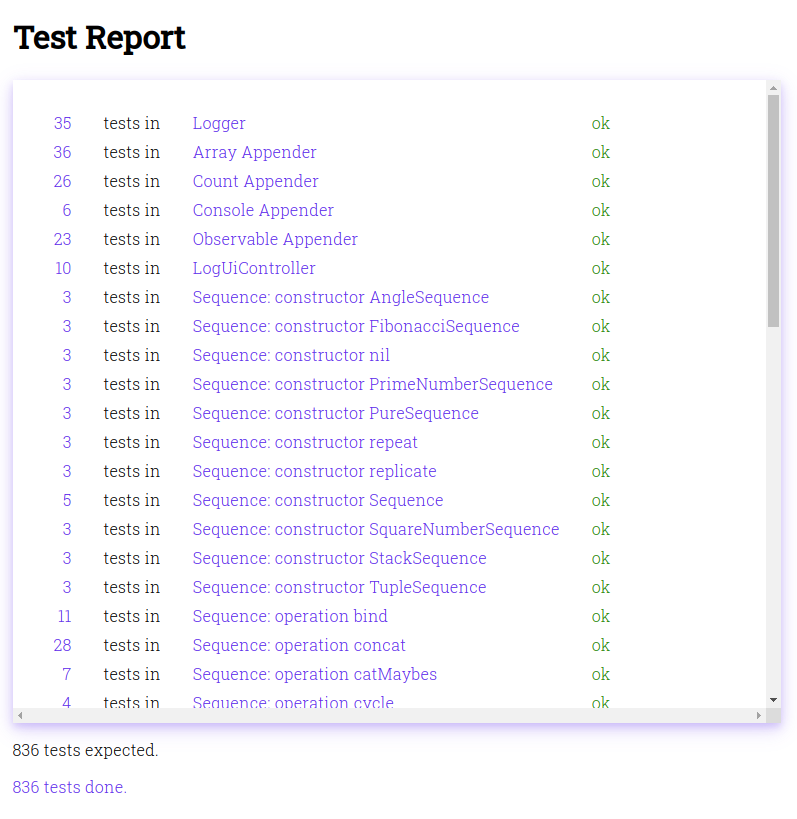
\includegraphics[width=0.8\textwidth]{mainmatter/pictures/test_report.png}
    \caption{Example Test Report}
    \label{fig:test_report}
\end{figure}


To demonstrate how to work with the |TestSuite|, examine the following
Listing~\ref{lst:testsuit_demo}:

\begin{lstlisting}[
  style=ES6, 
  caption=TestSuite demonstration,
  label={lst:testsuit_demo}
  ]
const suite = TestSuite("The truth");
suite.add("true is really true", assert => {
  assert.is(true, true);
});
suite.run();
\end{lstlisting}

Description of the functionalities: 

\begin{itemize}
  \item{|TestSuite|: A |TestSuite| contains the test cases and is identified by a
    name. This name represents the suite on the summary page on
  Figure~\ref{fig:test_report}when executing.}
  \item{|run|: executes all tests containing the |TestSuite|.}
  \item{|add|: A function for including a test case into the |TestStuite|. Its
      parameters are a string |name| and a callback which provides the test.}
\end{itemize}

\subsection{Additional Assertions}
\label{sub:Additional Assertions}

Assert functions in the Kolibri testing framework execute tests by comparing
two values and store the result in the summary collection of the |TestSuite|.
Listing~\ref{lst:testsuit_demo} shows the comparison of two |boolean|s using
|assert.is(...)| function.
This function compares an |actual| and an |expected| value. These two values
must match. Otherwise, the test fails.

\subsubsection{Assertion}
\label{subsub:Assertion for Iterables}
Comparing iterables is slightly more complicated. For this reason, we extended
the testing framework with an additional assert function that compares two
arbitrary iterables. Listing~\ref{lst:iterableEq} shows the usage of this
function called |iterableEq|:

\begin{lstlisting}[
  style=ES6, 
  caption=Usage of iterableEq,
  label={lst:iterableEq}
  ]
testSuite.add("demo iterableEq", assert => {
  const sequence = Sequence(0, x => x < 2, x => x +1);

  assert.iterableEq(sequence, [0,1]);
  assert.iterableEq(sequence, Pair(0)(1));
  assert.iterableEq(sequence, Range(1));
});  
\end{lstlisting}

The implementation of |iterableEq| is suitable for all different iterables.
Listing~\ref{lst:impl_iterableEq} shows the implementation of |iterableEq|:

\begin{lstlisting}[
  style=ES6, 
  caption=Implementation of iterableEq,
  label={lst:impl_iterableEq}
  ]
// test.js
...
iterableEq: (actual, expected, maxElementsToConsume = 1_000) => { *'\label{line:signature_iterableEq}'*

    if (actual[Symbol.iterator]   === undefined) error("..."); *'\label{line:check_iterable}'*
    if (expected[Symbol.iterator] === undefined) error("...");

    const actualIt     = actual[Symbol.iterator]();
    const expectedIt   = expected[Symbol.iterator]();

    let iterationCount = 0;
    let testPassed     = true;
    let message        = "";

    while (true) {
     const { value: actualValue,   done: actualDone  } = actualIt.next();
     const { value: expectedValue, done: expectedDone } = expectedIt.next();

     const oneIteratorDone      = actualDone || expectedDone;
     const bothIteratorDone     = actualDone && expectedDone;
     const tooManyIterations    = iterationCount > maxElementsToConsume;

     ... error handling omitted ...

     iterationCount++;
    }
    if (!testPassed) error(message);
    results.push(testPassed);*'\label{line:write_result_to_summary}'*
    messages.push(message);
}
\end{lstlisting}

The implementation checks on line~\ref{line:check_iterable} if both values are
iterable. If this is the case, each value of the two iterables is compared
using a |while| loop. On line~\ref{line:write_result_to_summary}, the
test stores the result into the summary collection of the corresponding |TestSuite|.
\newline
Since an |Itearble| can be endless, |iterableEq| defines a default maximum
iteration amount on line~\ref{line:signature_iterableEq}.  This is handy
because it is often the case that an |Iterable| runs infinitely while something
goes wrong. If an iterable exceeds this limit, the test fails.

\subsubsection{Assertion for Exceptions}
\label{subsub:Assertion for Exceptions}
Another extension for the Testing Framework is the |assert.throws| function.
It is often the case, that functions can throw an exception in a specific situation.
For example, such a case would be if we want to find the maximum on an empty
iterable. |max| throws an exception in this case. Therefore, testing the
function's behavior in error cases is also required. For this purpose, the
following Listing~\ref{lst:impl_throws} shows the implementation of |assert.throws|.

\begin{lstlisting}[
  style=ES6, 
  caption=Implementation of assert.throws,
  label={lst:impl_throws}
  ]
// test.js
...
throws: (functionUnderTest, expectedErrorMsg = "") => {
     let testResult    = false;
     let message       = "";
     const hasErrorMsg = expectedErrorMsg !== "";

     try {
         functionUnderTest();*'\label{line:functionToTest}'*
         message = "Did not throw an error!";
         if (hasErrorMsg) {
             message += ` Expected: '${expectedErrorMsg}'`;
         }
         error(message);
     } catch (e) {
         testResult = true;

         if (hasErrorMsg) {
             testResult = expectedErrorMsg === e.message;
         }
     }
     results .push(testResult);
     messages.push(message);
 }
 ...
\end{lstlisting}


Line~\ref{line:functionToTest} shows the call of the function under test. As
expected, this function should throw an exception that is caught in the catch
block. If this is the case, the test is successful. Otherwise, the test fails
and a corresponding error message is stored.

\section{Testing Table}
\label{sec:Testing Table}
This Section describes the realization of the testing table. It examines the
architecture of it and how it works for a particular operation. It covers the
config-based testing approach, which enables generalizing test cases for the
Sequence library.

The architecture consists of three main parts:
\begin{itemize}
  \item{A table containing all testing functions.}
  \item{Configuration objects to define test properties.}
  \item{A function |addToTestingTable| which includes all tests from the testing
    table into a given |TestSuite|.}
\end{itemize}

Each constructor and operator of the Sequence library has its configuration
that specifies the test behavior. Likewise, each has its |TestSuite|. 
The following sections address the different parts separately.

\subsection{The Table}
\label{sub:The Table}
The testing table is just an array (table) containing test objects.
Each object consists of two properties. Listing~\ref{lst:testing_table} shows
the implementation.

\begin{lstlisting}[
  style=ES6, 
  caption=Testing Table,
  label={lst:testing_table}
  ]
const testingTable = [
  { name: TESTS.TEST_SIMPLE,                   test: testSimple},
  { name: TESTS.TEST_PURITY,                   test: testPurity},
  { name: TESTS.TEST_CB_NOT_CALLED_AFTER_DONE, test: testCBNotCalledAfterDone},
  { name: TESTS.TEST_PROTOTYPE,                test: testPrototype},
  { name: TESTS.TEST_INVARIANTS,               test: testInvariants},
  { name: TESTS.TEST_ITERATE_MULTIPLE_TIMES,   test: testIterateMultipleTimes},
];
\end{lstlisting}

An object in the table includes two properties:
\begin{itemize}
\item{A string representing its name. The name is important for displaying an accurate error message if the test fails.}
\item{A function to test a specific behavior}
\end{itemize}

Each function of the testing table expects as argument a test configuration
object of type |SequenceTestConfigType|.
Listing~\ref{lst:test_simple} presents exemplary the implementation of |testSimple|.

\begin{lstlisting}[
  style=ES6, 
  caption=Implementaion Test Simple,
  label={lst:test_simple}
  ]
/**
 * @type {
 *             (config: SequenceTestConfigType)
 *          => (assert: AssertType)
 *          => void
 *       }
 */
const testSimple = config => assert => {
  const { iterable, operation, evalFn, expected, param } = config;*'\label{line:test_config_destructuring}'*
  const baseIterable = iterable(); *'\label{line:test_config_iterable}'*
  const operated     = operation(param)(baseIterable);*'\label{line:test_config_operated}'*
  evaluate(expected, operated, assert, evalFn);*'\label{line:test_config_eval}'*
};
\end{lstlisting}

The function |simpleTest| examines whether an operation correctly processes a typical use case.
For this purpose, the following tasks are executed: 
\begin{itemize}
  \item{Line~\ref{line:test_config_iterable} shows the invocation of
    iterable to yield an |Iterable| for further use.}
  \item{Line~\ref{line:test_config_operated} executes the operation by passing
    the required parameters. This is an optional configuration parameter
  |param|, like a predicate, and an |Iterable|.}
  \item{Line~\ref{line:test_config_eval} compares the |actual| and |expected| value with a given eval function. } 
\end{itemize}

The testing table includes test-functions to examine the following behaviors of
implementations of the Sequence library:

\begin{itemize}
  \item{\textbf{testSimple} checks if a typical case works properly.}
  \item{\textbf{testPurity} checks if an |operator| makes some side effects.}
  \item{\textbf{testCBNotCalledAfterDone} checks if a given callback of an
    |operator| will be called when the |Iterable| is exhausted.}
  \item{\textbf{testPrototype} checks if the SequencePrototype is set.}
  \item{\textbf{testInvariants} checks if an invariant holds by applying different parameters.}
  \item{\textbf{testIterateMultipleTimes} checks if an |Iterable| produces the same output twice.}
\end{itemize}


\subsection{Running the Testing Table}
\label{sub:Running the Testing Table}
|addToTestingTable| inserts the tests of the testing table into the |TestSuite| for a
specific configuration, visible on line~\ref{line:add_to_testsuite}. 
Since the configuration runs all tests of the testing table by default, it
must provide an option to exclude tests for exceptional cases. 
Line~\ref{line:filtering_tests} filters out all excluded tests.
This mechanism is necessary because specific tests do not make sense for 
particular operators and constructors. For example, if an operation has no
callback, the check of its side effect is useless.

\begin{lstlisting}[
  style=ES6, 
  caption=The addToTestingTable function,
  label={lst:impl_addToTestingTable}
  ]
export { addToTestingTable }
...
/**
 * @type {
 *       (testSuite: TestSuiteType)
 *    => (config: SequenceTestConfigType)
 *    => void
 * }
 */
const addToTestingTable = testSuite => config => {
  const { excludedTests } = config;

  testingFunctions
    .filter (({ name })        => !excludedTests.includes(name)) *'\label{line:filtering_tests}'*
    .forEach(({ name, test })  => 
         testSuite.add(`${name}: ${config.name}`, test(config)));*'\label{line:add_to_testsuite}'*
};
\end{lstlisting}

\subsection{Configuring the Testing Table}
\label{sub:Configuring the Testing Table}

In order to test operators and constructors using the testing table, it is
necessary to implement a test configuration.
Listing~\ref{lst:config_reduce} shows the configuration of |reduce|. 
Line~\ref{line:start_test_config} to~\ref{line:end_test_config} defines the test 
configuration for |reduce|. Each configuration has its own |TestSuite|. Therefore, it is possible to add
some tests for special cases not covered by the table on line~\ref{line:additional_test_cases}.


\begin{lstlisting}[
  style=ES6, 
  caption=Test configuration reduce,
  label={lst:config_reduce}
  ]
const testSuite = TestSuite("Sequence: terminal operation reduce$");

addToTestingTable(testSuite)(*'\label{line:start_test_config}'*
  createTestConfig({*'\label{line:createTestConfig}'*
    name:      "reduce$",
    iterable:  () => newSequence(UPPER_SEQUENCE_BOUNDARY),
    operation: () => reduce$((acc, cur) => acc + cur, 0),
    expected:  10,
    evalFn:    expected => actual => expected === actual,
    excludedTests: [TESTS.TEST_CB_NOT_CALLED_AFTER_DONE]
  })
);*'\label{line:end_test_config}'*


testSuite.add("test: special case", assert => {*'\label{line:additional_test_cases}'*
  // Given
  // When
  // Then
});

testSuite.run();
\end{lstlisting}

On line~\ref{line:createTestConfig}, the function |createTestConfig| ensures
that required properties are set using notation. Furthermore, it sets default
values of configuration properties to simplifying the code.

The following Table~\ref{tab:testing_table} shows which configuration 
properties are available and the purpose of it:


\begin{table}[H]
  \center
  \begin{tabular}{ l m{10cm} c}
    \textbf{Property} & \textbf{Description} & \textbf{Required}\\
    \hline
    |name|            & The name of the |Iterable| under test for meaningful 
                      report messages. 
                    & y 
                    \\ 
    |iterable|        & A function that constructs a new |Iterable| to apply the 
                      operation to. 
                    & y 
                    \\  
    |expected|        & The expected result of the operation applied to the |Iterable|
                      defined in property |iterable|.
                    & 
                    y  \\ 
    |excludedTests|   & An optional array of |TestingFunction| to exclude tests
                      in testing table. 
                    & n 
                    \\
    |operation|       & The operation to test. |param| is passed as an argument
                      to it
                     (leave this empty for constructor 
                      tests since they do not take an inner iterator). 
                    & n 
                    \\
    |param|           & A parameter passed to this |operation|. If it is a
                      function, some extra tests will be performed. 
                    & n
                    \\ 
    |invariants|      & An optional array of |InvariantCallback|. The invariant 
                      must hold tests against different lists. 
                    & n
                    \\
    |evalFn|          & An optional function that takes |expected| and the |actual| 
                      in curried style. The default is |iterableEq|.
                    & n 
                    \\
  \end{tabular}
  \caption{Properties of the configuration object}
\label{tab:testing_table}
\end{table}


\section{Testing based on Properties}
\label{sec:Testing based on Properties}
John Huges and Carl Claessen wrote to following sentence in the paper
"Quickcheck, A Lighweight Tool for Random Testing of Haskell Programms":
\textit{
Despite anecdotal evidence that functional programs require somewhat less
testing (`Once it type-checks, it usually works'), in practice it is still a 
major part of functional program development}~\cite{quickcheck_hughes}.
If these programming icons claim it takes many tests even in a strongly typed 
language, how many does it take in JavaScript? Of course, enough.

\subsection{Invariant Testing}
\label{sub:Invariant Testing}
We added another kind of tests to increase the Sequence library's robustness -
invariant testing. Some aspects of this testing are leaned on the Quickcheck
approach of the paper mentioned before. We concentrated on only some essential
parts since we cannot implement a whole Quickcheck framework in this work.
\newline
In the test configuration object
is a property |invariant|s available. It allows defining of some invariants, which are
tested with different parameters. Quickcheck does this with randomly generated
data. Our data is fixed and includes a mix of typical a special cases.
\newline
Listing~\ref{lst:test_config_reverse} show the test configuration of |reverse|.

\begin{lstlisting}[
  style=ES6, 
  caption=Test Configuration reverse,
  label={lst:test_config_reverse}
  ]
const testSuite = TestSuite("Sequence: operation reverse$");

addToTestingTable(testSuite)(
  createTestConfig({
    name:      "reverse$",
    iterable:  () => newSequence(UPPER_SEQUENCE_BOUNDARY),
    operation: () => reverse$,
    expected:  [4, 3, 2, 1, 0],
    invariants: [
    it => reverse$(reverse$(it)) ["=="] (it), *'\label{line:reverse_law}'*
    ]
  })
);

testSuite.run();
\end{lstlisting}
On line~\ref{line:reverse_law} in Listing~\ref{lst:test_config_reverse} we can 
see the definition of an invariant. This statement defines that an iterable must be 
equal to the original when reversed two times.
\newline
The testing table contains a test function |testInvariants|. This function is on
Listing~\ref{lst:invariant_penetration} below.

\begin{lstlisting}[
  style=ES6, 
  caption=Implementation invariant penetration,
  label={lst:invariant_penetration}
  ]
/**
 * Applies a series of lists to a given invariant.
 * @template _T_
 * @type {
 *            (invariants: InvariantCallback)
 *         => (assert: AssertType)
 *         => void
 *       }
 */
const invariantPenetration = invariant => assert => {
  const testingLists = [ *'\label{line:list_of_parameters}'*
    // edge case
    nil,                                                   
    // edge case, done calculated
    newSequence(1),                                        
    // typical number
    newSequence(3),                                        

    // no big iterable, needs extra test

    // edge case, done set explicitly
    PureSequence("testString"),                            
    // mixing types
    ['a', 'b', 'c', 1, 2, 3, Nothing, Just("testString")], 
    // iterable of iterables
    [PureSequence(1), newSequence(4), '#', "abc", 1]       
  ];

  for (const list of testingLists) {
    const result = invariant(list);
    assert.isTrue(result);
  }
};
\end{lstlisting}

Line~\ref{line:list_of_parameters} defines a list with several parameters of
type |Iterable|. Each parameter tests if the invariant of |reverse| holds. 
This enables for testing many cases written in a few lines of code.

\subsubsection{An advanced Example}
\label{subsub:An advanced Example}
In the following we will look at the laws of the operation |mconcat|, which
flattens an iterable of iterables. If |mconcat| follows certain laws, the
sequence forms a monoid under this operation.~\cite{haskell_monoid}
Listing~\ref{lst:lr_identity_mconcat} shows the definition of the identity law:

\begin{lstlisting}[
  style=Haskell,
  caption=Left and right identity of mconcat,
  label={lst:lr_identity_mconcat}
]
-- left identity
x <> mempty = x
-- right identity
mempty <> x = x
\end{lstlisting}

The |<>| operator is defined on the semigroup, a monoid subset. The binary 
operator |<>| is associative and concatenates two lists.
Listing~\ref{lst:lr_identity_mconcat} demonstrates that a list $x$ concatenated
with |nil|, the empty list, equals the original one. With our implementation of
the invariants, we can now represent and test the laws similarly.
Listing~\ref{lst:mconcat_invariant} shows the implementation.

\begin{lstlisting}[
  style=ES6, 
  caption=Invariants of mconcat,
  label={lst:mconcat_invariant}
  ]
addToTestingTable(testSuite)(
  createTestConfig({
    name:       "mconcat",
    iterable:   () => 
      toMonadicIterable([ newSequence(2), newSequence(2), newSequence(2) ]),
    operation:  () => mconcat,
    expected:   [0, 1, 2, 0, 1, 2, 0, 1, 2],
    invariants: [
      it => mconcat([nil, it]) ["=="] (it),*'\label{line:mconcat_first_invariant}'*
      it => mconcat([it, nil]) ["=="] (it),*'\label{line:mconcat_second_invariant}'*
      it => [...mconcat([PureSequence(1),it])].length > [...it].length,
    ],
  })
)
\end{lstlisting}

Let us focus on line~\ref{line:mconcat_first_invariant} and 
\ref{line:mconcat_second_invariant}.
The property |invariants| expect an array of functions. Each of these
functions represents a law. Therefore, the function injects an arbitrary list
called |it|, and the law must hold for it. In the same way, this provides the
ability to check other implementation-specific behavior.

\subsection{Revealed Code Bugs: Discoveries through Testing during Development}
\label{sub:Revealed Code Bugs: Discoveries through Testing during Development}
This section focuses on the enhancements made by the testing framework. As
illustrated in the Table section, a test case named |TEST_CB_NOT_CALLED_AFTER_DONE|
guarantees that a callback is not invoked once an iterator is exhausted. This
test arose from a realization during development that it is expected for a
callback not to be called after the iterator is used up. Such occurrences could
lead to program errors or unexpected behavior. Consequently, we implemented a
test case addressing this scenario and added it to the TestingTable. By adding
just one more test, the entire Sequence Library could be examined for this
behavior, allowing for further improvements.
\\
Another example concerns the behavior of operators and operations when dealing
with empty iterables. The inclusion of invariant tests automatically contains the
scenario involving an empty iterable. Other cases involving special iterables
can also be tested, helping prevent other errors.
\\
Furthermore, another special test case is the |TEST_PURITY|, which ensures that
the state of an iterable is in the proper location. This safeguards against
unexpected side effects, promoting a more reliable program execution.

\subsection{Conclusion}
\label{sub:Conclusion}
When implementing large code bases, it is crucial to have a solid test
framework. This framework has to be continuously extended and improved during
development.
Handling a rising number of cases during development leads to testing the core
functionality in various ways, making the core even more stable.
\newline
The standardization and generalization of tests using a testing table imply that
writing tests for new functionalities takes less time and ensures better
quality.
